\chapter{Sequence diagrams}
\section{Business}
The businness layer isn't supposed to know about the view. As seen in figure \ref{fig:seqbus} the \emph{MainWindow} is not visible, so the message comes from 'somewhere'. Then it will do some bushiness logic like checking if a component would not be overlapping another component. At the end when the flow network has changed the changes will be send back using callbacks to the presentation layer.

\section{Overall}
In figure \ref{fig:seqoverall} a sequence diagram is visible which goes through all the layers of the application. Very noticeable is that \emph{IFlowModel} and \emph{IDataAccesLayer} both have the \emph{OpenFile} operation. Usually the presentation layer isn't suppose to know about the data layer because the data access layer usually contains CRUD operations.

\section{Presentation layer}
The sequence diagram in figure \ref{fig:seqprespipe} only contains the MVC pattern since no \emph{ViewModel} is used. Many steps are required to get the selected component on the screen since the standard graphics are used.

\begin{figure}[h!]
	\centering
	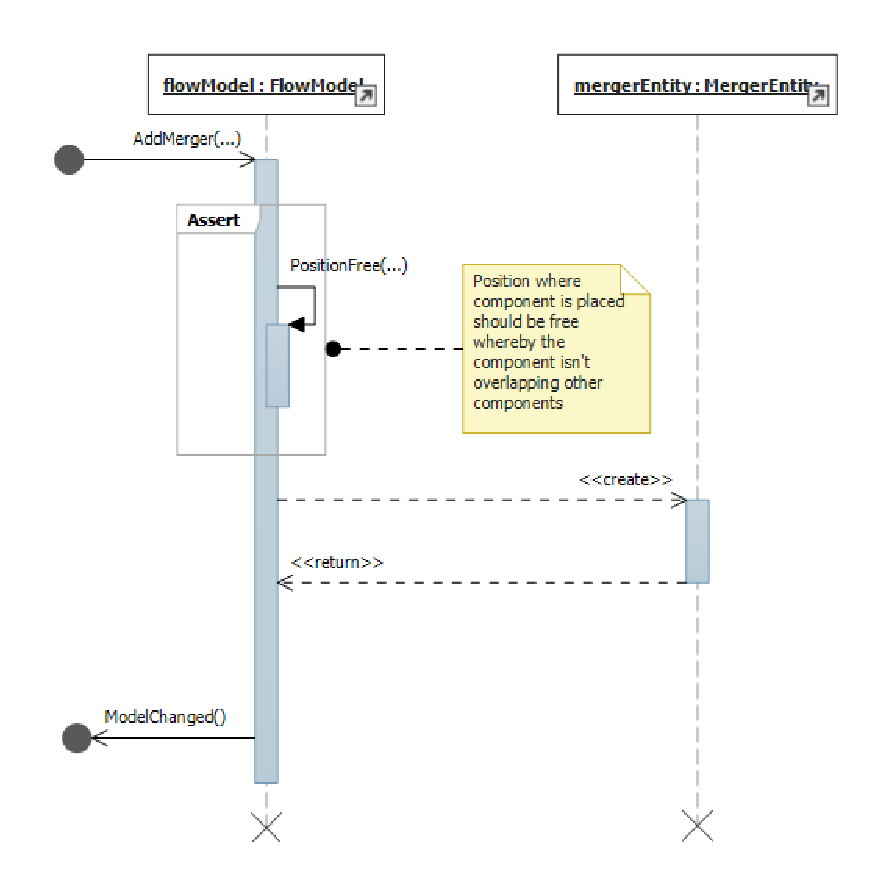
\includegraphics{figures/BusinessAddNewComponent.pdf}
	\caption{Business add new component}
	\label{fig:seqbus}
\end{figure}

\begin{figure}[h!]
	\centering
	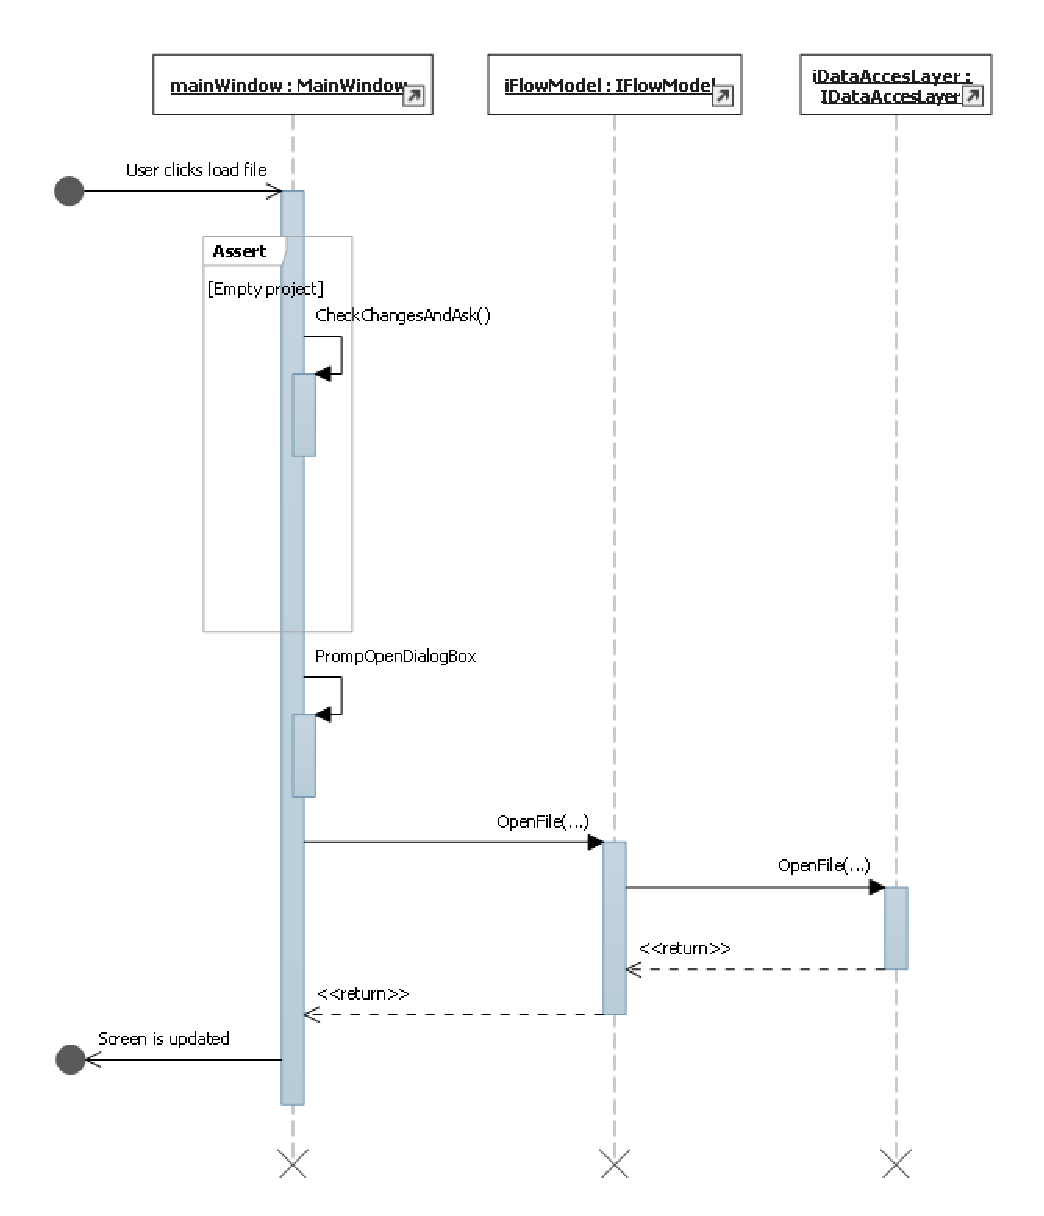
\includegraphics[width=\textwidth]{figures/OverallLoadFile.pdf}
	\caption{Overall load file}
	\label{fig:seqoverall}
\end{figure}

\begin{sidewaysfigure}[h!]
	\centering
	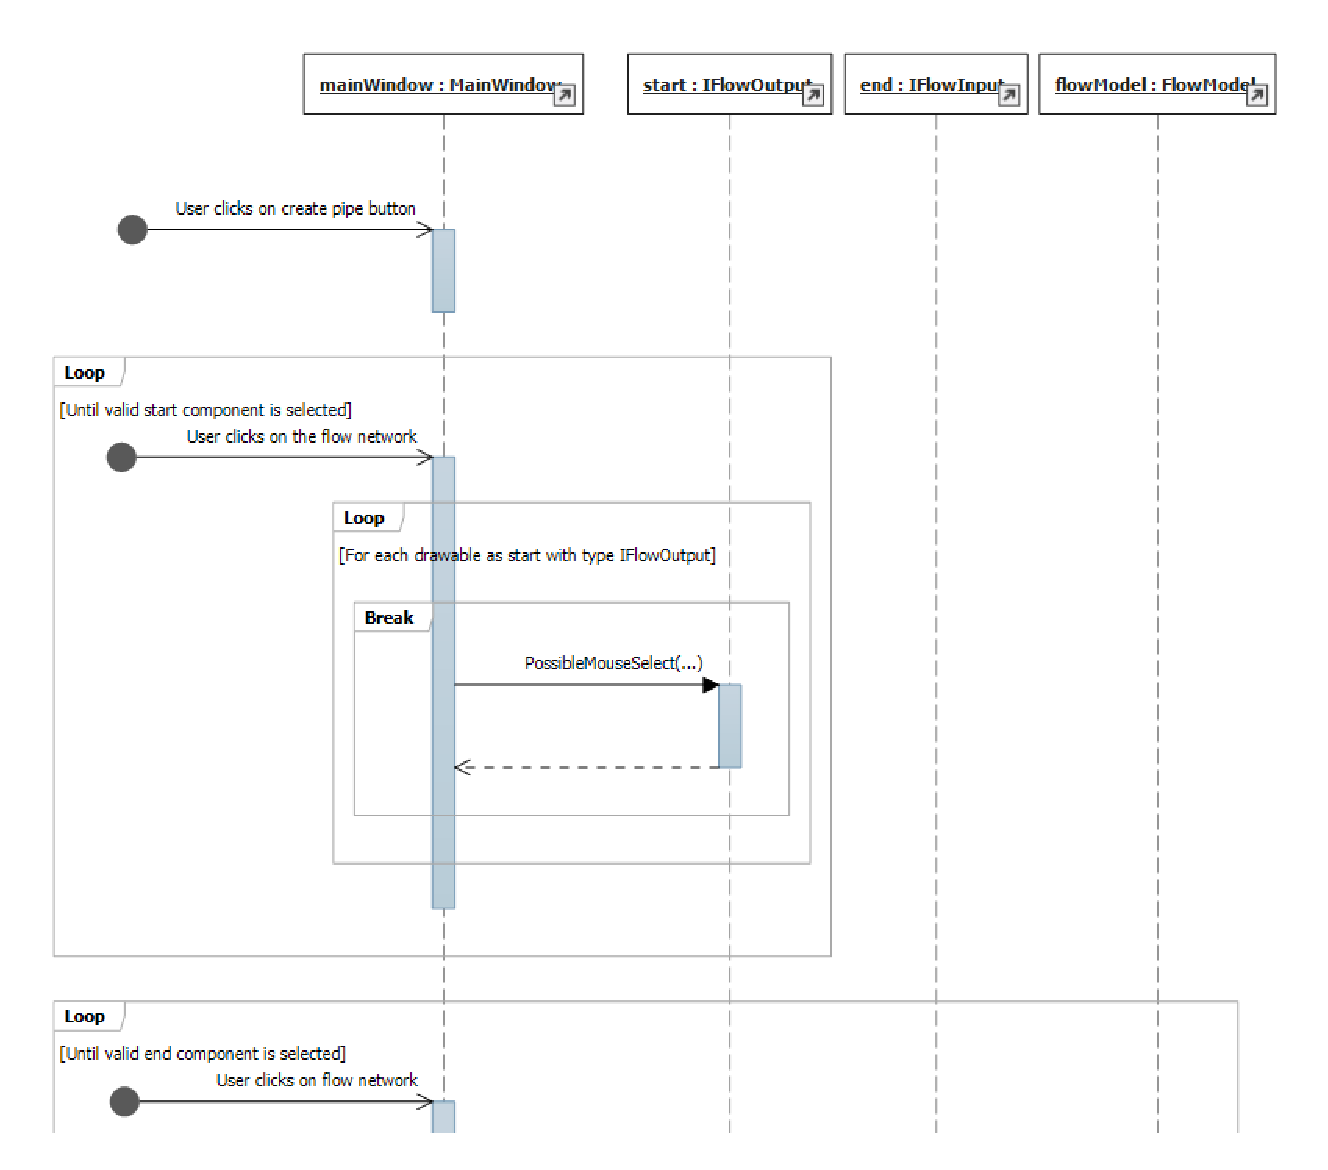
\includegraphics[width=\textwidth]{figures/PresentationCreateConnection1.pdf}
	\caption{Presentation create pipeline}
	\label{fig:seqprespipe}
\end{sidewaysfigure}

\begin{sidewaysfigure}[h!]
	\centering
	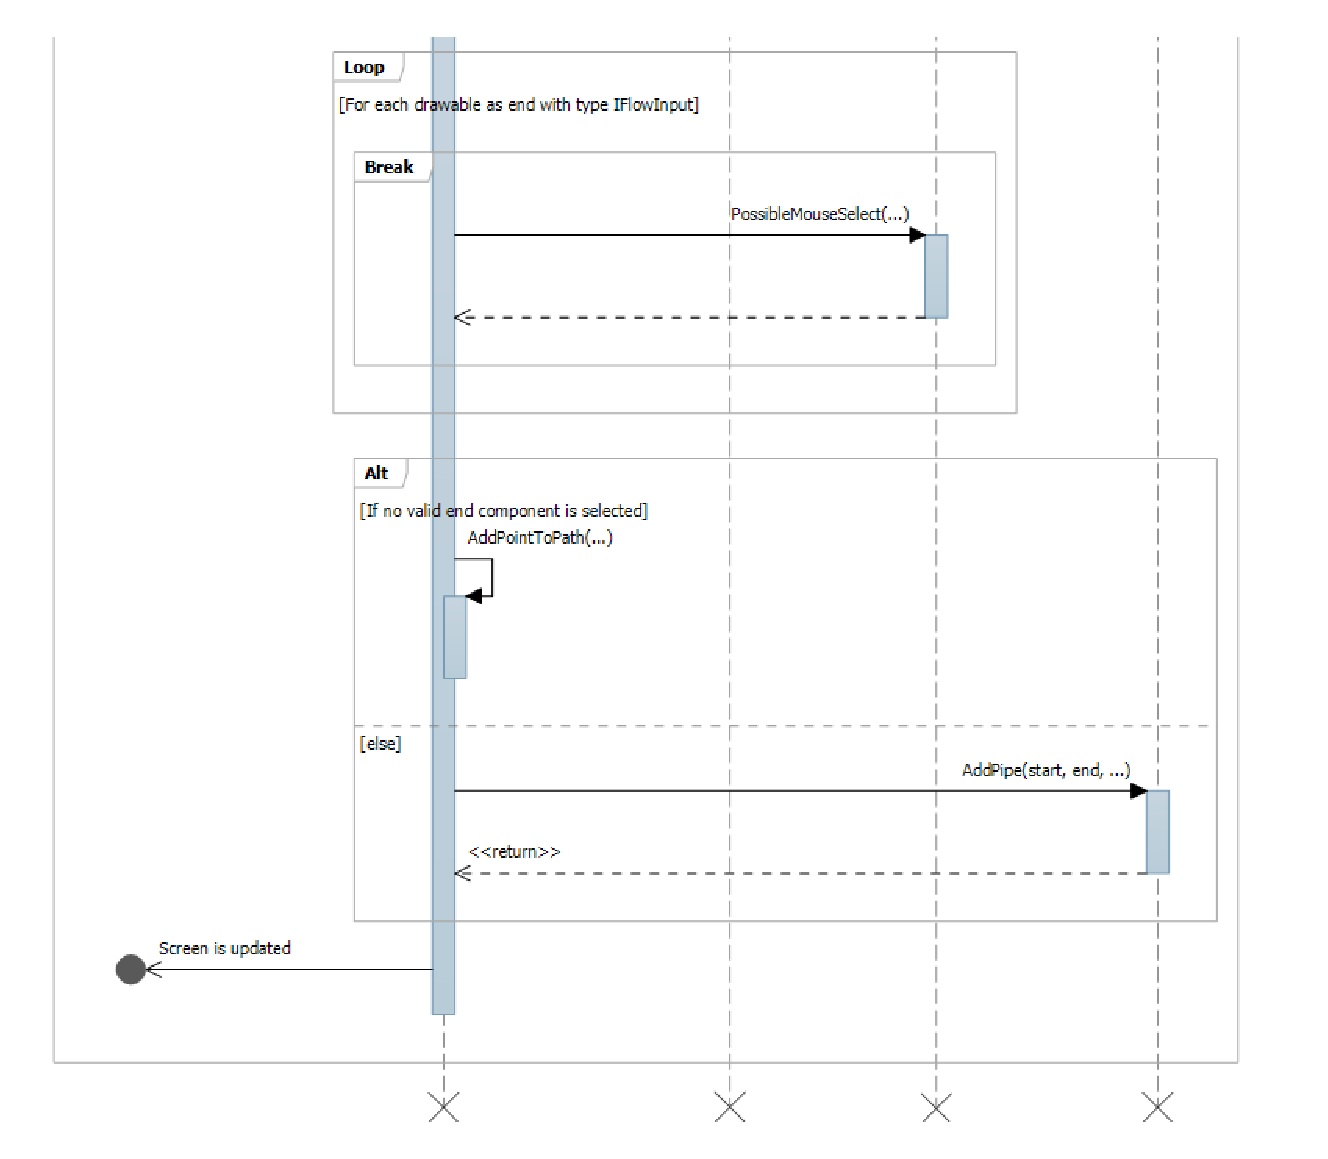
\includegraphics[width=\textwidth]{figures/PresentationCreateConnection2.pdf}
\end{sidewaysfigure}